Figure \ref{fig:tesearch} shows the comparison of all possible combinations of temporal embeddings on ML-1M and Amazon Game dataset. We fixed all other hyperparameters (e.g., $h=60$). Interestingly, the importance of each embedding seems to differ in each dataset. In ML-1M, relative position embeddings (especially \textbf{Log}) seem to play an important role, whereas in Amazon Game, absolute position embeddings (especially \textbf{Day}) seem to be essential. Therefore, the optimal combination is also different for each dataset. Further analysis with different $h$ shows us that while optimal combination differs slightly for each $h$, the overall tendency stays the same for each dataset. The same applies to other datasets. This suggests that datasets with distinct characteristics require carefully chosen temporal embeddings that provide the right views on the context of user-item interactions. Note that while we only used $n=2\text{ and }4$ for Table \ref{tab:results} to be fair with other baselines, using all possible $n$ can further improve our performance.
% EH: 아래와 같은 문장 정도면 어떨까 
%When we apply the same analysis on the different datasets, the best joint set of embeddings is different. According to our observation, each dataset has unique contextual characteristics which is useful information to predict the next behavior. 
%This suggests that datasets with different characteristics require different view on the positions of user-item interactions in a sequence. [ANALYZE WHY]

% In this section we seek to study the effect of various positional embeddings. To assess the contribution of each positional embedding type in more detail, we ran an extensive experiment to test all combinations of positional embeddings. Figure-\ref{fig:tesearch} shows the comparison of NDCG@10 performance on ML-1M and Amazon Game dataset. All other hyperparameters were kept equal.

% \begin{figure}[ht]
  \centering
  \begin{subfigure}[ht]{.49\linewidth}
    \centering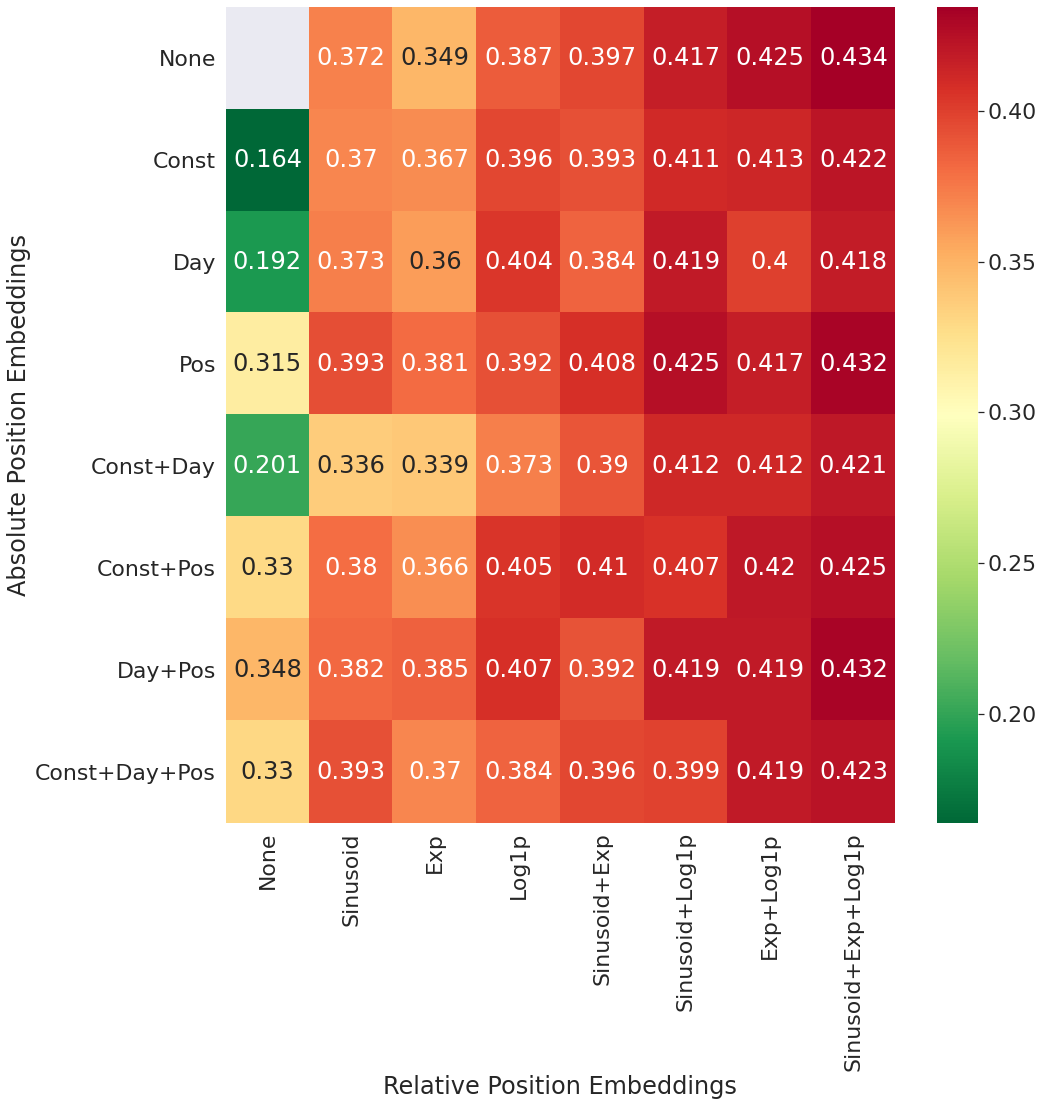
\includegraphics[width=.95\linewidth]{figures/tesearch.png}
    \caption{MovieLens 1M}
  \end{subfigure}
  \begin{subfigure}[ht]{.49\linewidth}
    \centering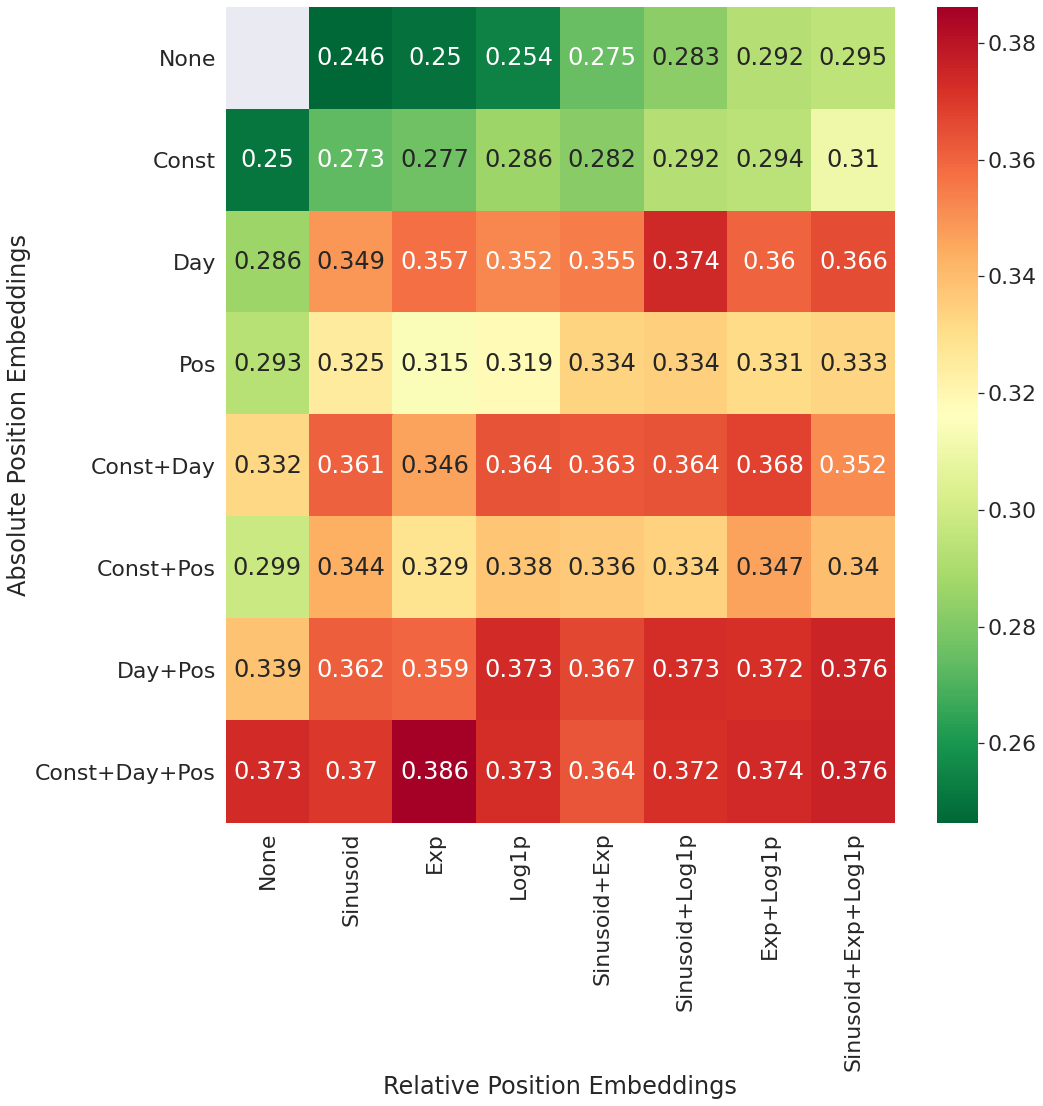
\includegraphics[width=.95\linewidth]{figures/tesearch_game.png}
    \caption{Amazon Game}
  \end{subfigure}
  \caption{NDCG@10 Comparison with All Possible Combinations of Positional Embeddings on ML-1M and Game Dataset}
  \Description{TODO:Description}
  \label{fig:tesearch}
\end{figure}

% Interestingly, the importance of each embedding seems to differ in each dataset. In ML-1M, relative position embeddings(especially \textbf{Log1p}) seem to play an important role, whereas in Amazon Game, absolute position embeddings(especially \textbf{Pos} and \textbf{Day}) seem to be essential. In ML-1M, the optimal performance is achieved when we use all three relative position embeddings and none of the absolute position embeddings. In contrast, using all three absolute position embeddings with only \textbf{Exp} relative embedding works best in Amazon Game. This proves that datasets with different characteristics require different view on the positions of user-item interactions in a sequence.

% %\begin{figure}[ht]
  \centering
  
  \begin{subfigure}[ht]{.33\linewidth}
    \centering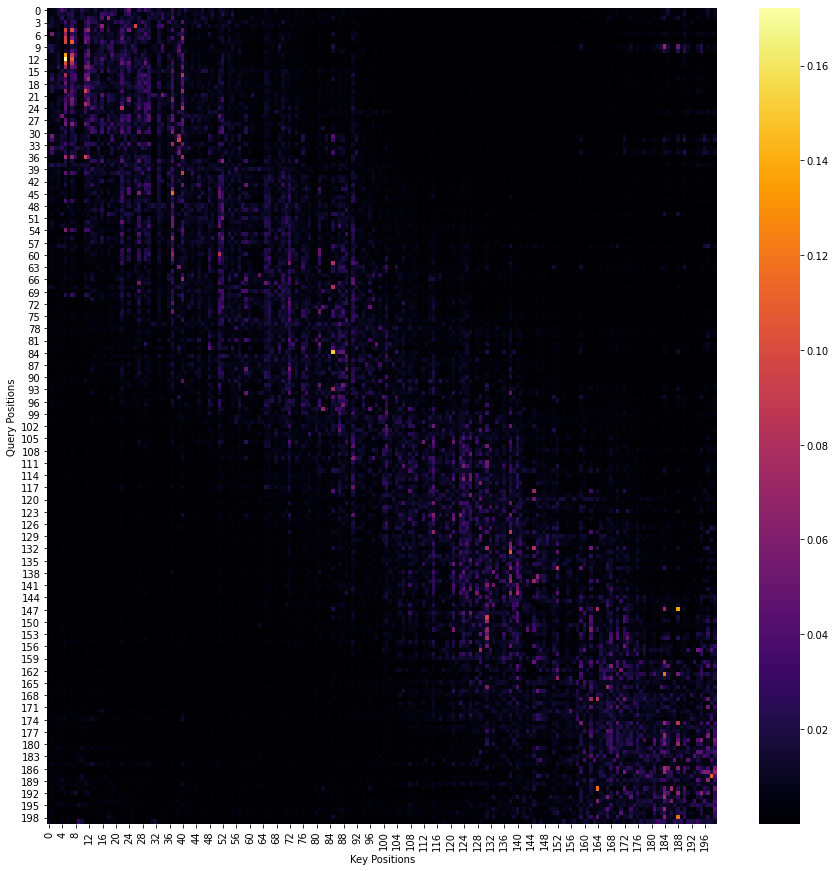
\includegraphics[width=.95\linewidth]{figures/attn1/L0BPH1.png}
    \caption{\textbf{Pos} Layer 0 Head 1}
  \end{subfigure}
  \begin{subfigure}[ht]{.33\linewidth}
    \centering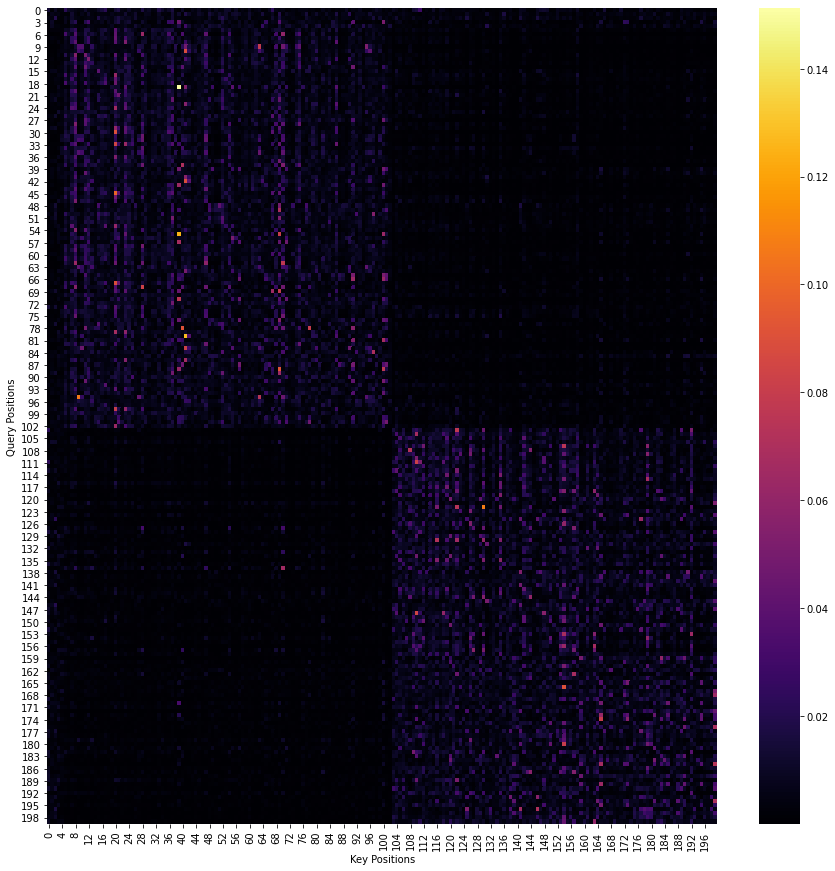
\includegraphics[width=.95\linewidth]{figures/attn1/L0BDH0.png}
    \caption{\textbf{Day} Layer 0 Head 0}
  \end{subfigure}
  \begin{subfigure}[ht]{.33\linewidth}
    \centering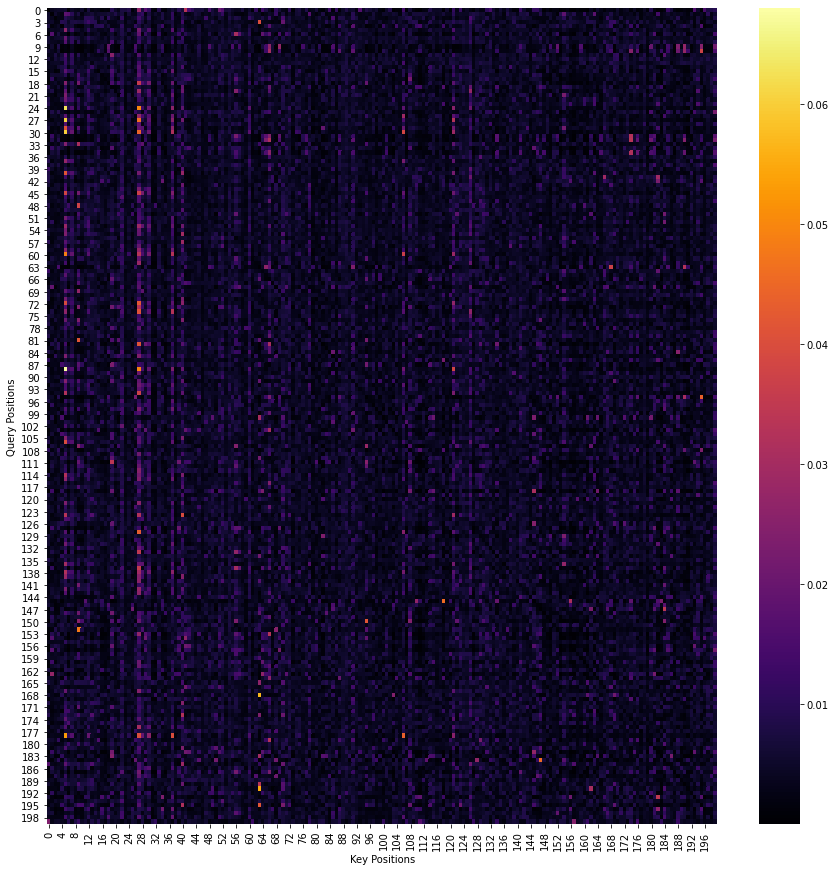
\includegraphics[width=.95\linewidth]{figures/attn1/L0BCH0.png}
    \caption{\textbf{Const} Layer 0 Head 0}
  \end{subfigure}
  \begin{subfigure}[ht]{.33\linewidth}
    \centering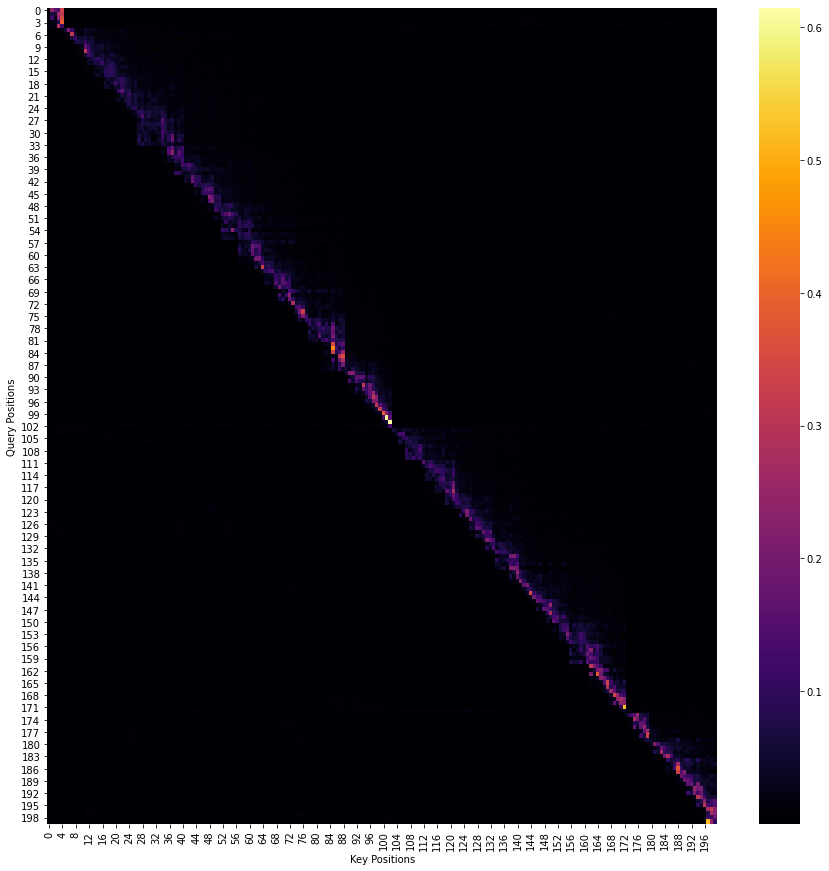
\includegraphics[width=.95\linewidth]{figures/attn1/L0BSH0.png}
    \caption{\textbf{Sinusoid} Layer 0 Head 0}
  \end{subfigure}
  \begin{subfigure}[ht]{.33\linewidth}
    \centering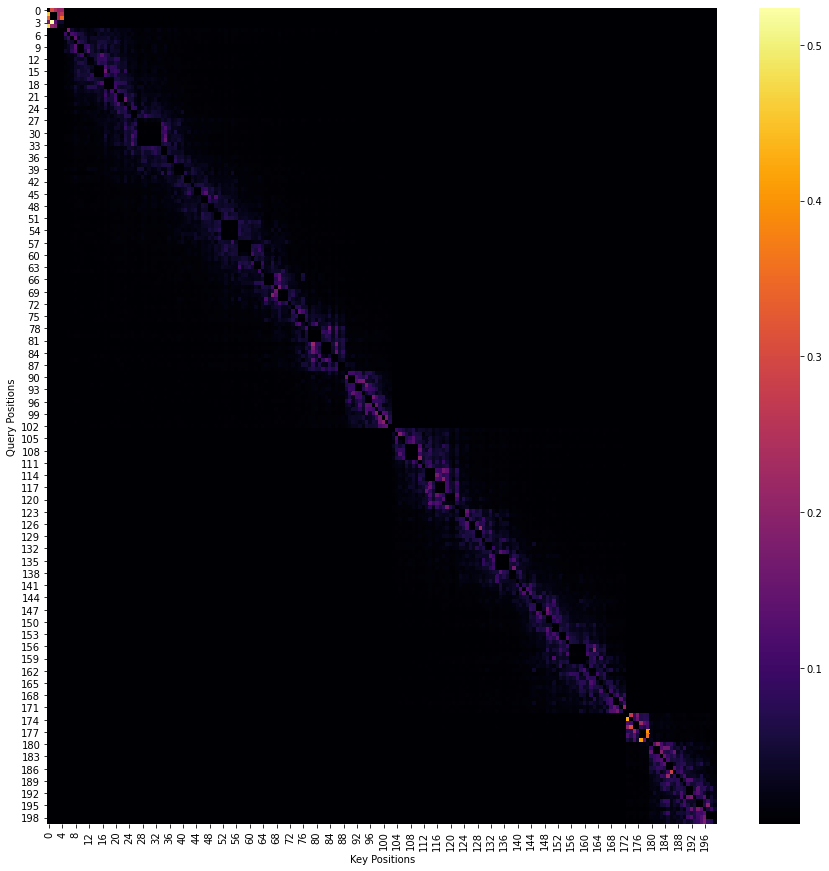
\includegraphics[width=.95\linewidth]{figures/attn1/L0BEH0.png}
    \caption{\textbf{Exp} Layer 0 Head 0}
  \end{subfigure}
  \begin{subfigure}[ht]{.33\linewidth}
    \centering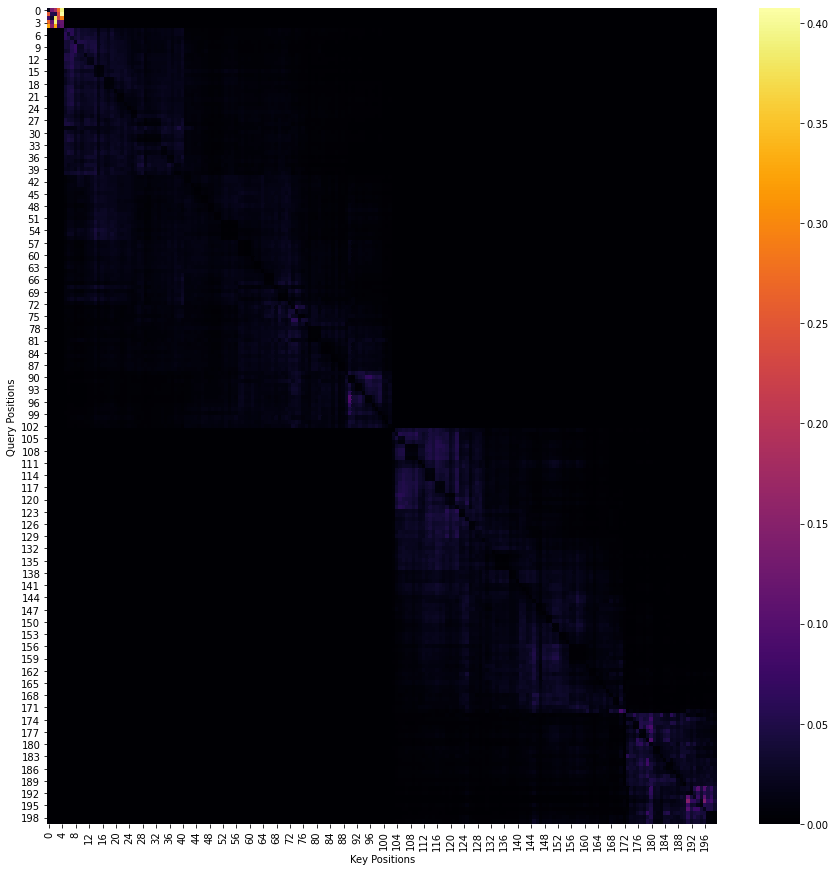
\includegraphics[width=.95\linewidth]{figures/attn1/L1BLH0.png}
    \caption{\textbf{Log1p} Layer 1 Head 0}
  \end{subfigure}
  
  %\subfigure{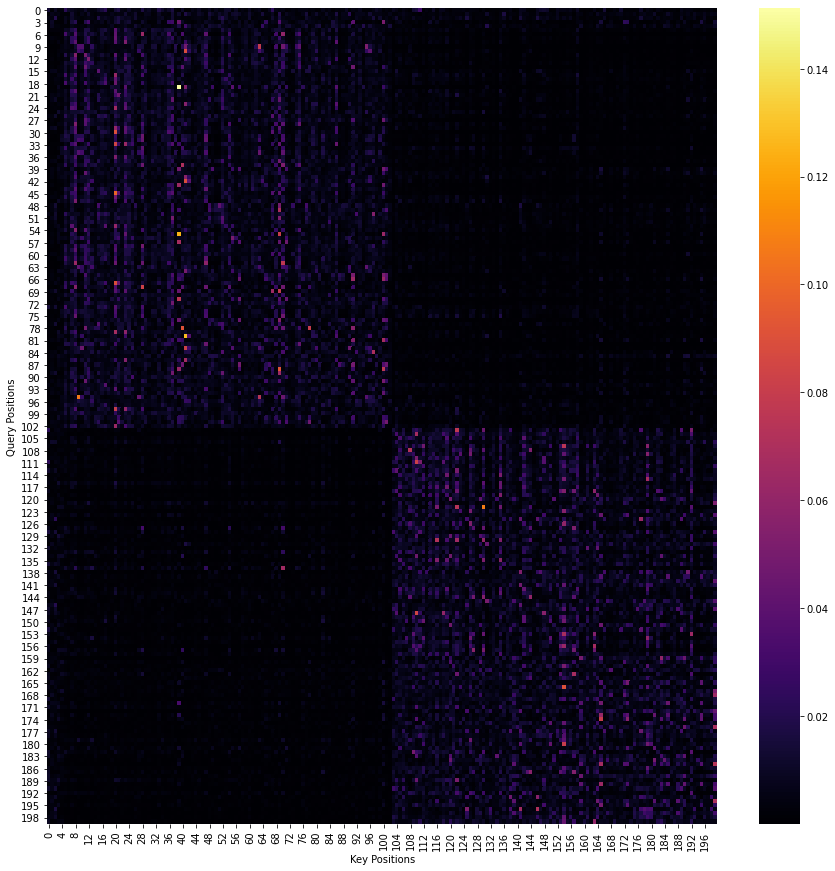
\includegraphics[width=0.5\linewidth]{figures/attn1/L0BDH0.png}}
  %\subfigure{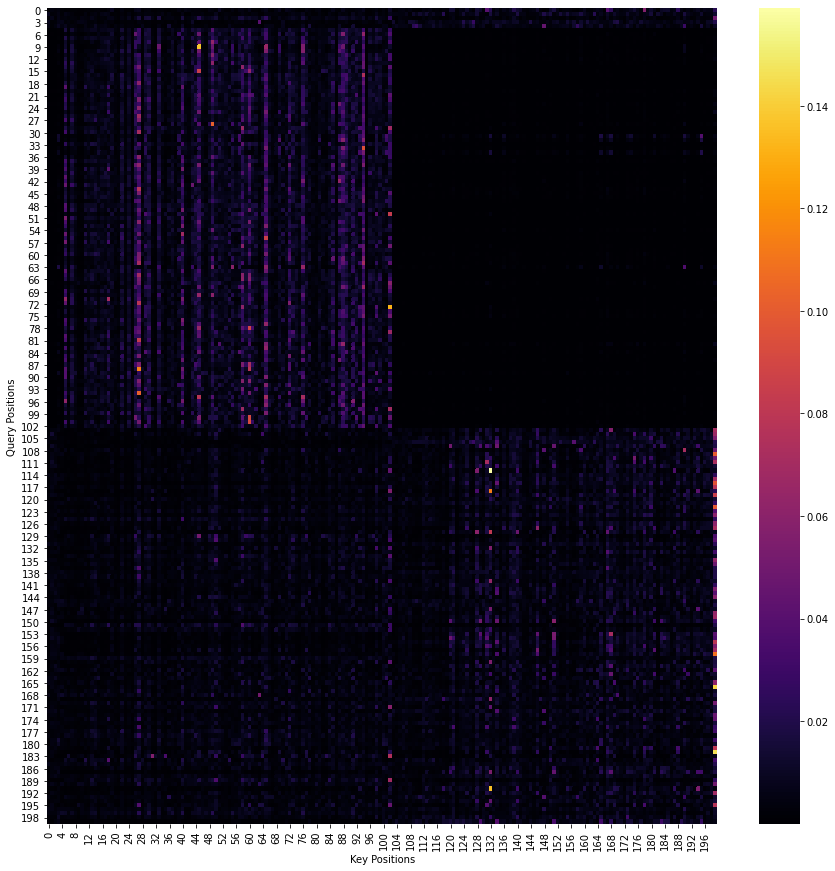
\includegraphics[width=0.5\linewidth]{figures/attn1/L0BDH1.png}}
  \caption{Attention Score Maps (Might need to change the figures to ones with shorter sequences (so that they are more clear))}
  \Description{TODO:Description}
  \label{fig:attnmaps}
\end{figure}

% \begin{table}[ht]
\caption{Gradient Comparison for Each Embedding Type}
\label{tab:grad_cam}
\begin{tabular}{@{}lllllll@{}}
\toprule
{Dataset} & {Pos}           & {Day}              & {Const}            & {Sinusoid}         & {Exp}           & {Log1p}         \\ \midrule
{ML1M}    & {4.79\%}        & {5.34\%}           & {1.50\%}           & {\textbf{51.34\%}} & {7.08\%}        & {\underline{29.94\%}} \\
{ML20M}   & {\underline{19.60\%}} & {5.50\%}           & {6.11\%}           & {\textbf{24.51\%}} & {\underline{22.58\%}} & {\underline{21.70\%}} \\
{Beauty}  & {1.03\%}        & {8.39\%}           & {\textbf{57.12\%}} & {9.79\%}           & {0.69\%}        & {\underline{22.98\%}} \\
{Game}    & {\underline{40.39\%}} & {\textbf{49.57\%}} & {1.96\%}           & {1.19\%}           & {1.37\%}        & {5.51\%}  \\ \bottomrule
\end{tabular}
\end{table}

% To further measure the contributions of each embedding type, we applied a method similar to Grad-CAM\cite{GRADCAM} to our fully equipped model(with all 6 embedding types). For every sequence in the test data, we took the output from the final layer of our self-attention block stacks $\mathbf{Z}^L = [\mathbf{Z}^L_1, ..., \mathbf{Z}^L_\Sigma]$, and then computed the gradient of each output with regard to the answer item's logit $y^c$:
% \begin{equation}
%     g_i = \frac{dy^c}{dZ^L_i}
% \end{equation}
% Similar to \cite{GRADCAM}, we only took positive gradients from $g_i$ to measure their positive influence on the answer's logit. We calculated the average of their sums and then applied softmax to get Table-\ref{tab:grad_cam}.

% As we expected, relative position embeddings were dominant in MovieLens datasets, while absolute position embeddings were dominant in Amazon datasets. Moreover, as we saw in Figure-\ref{fig:tesearch}-(b), \textbf{Pos} and \textbf{Day} play very important roles in Amazon Game. Unlike Figure-\ref{fig:tesearch}-(a), \textbf{Sinusoid} seems to be more influential than \textbf{Log1p} in ML-1M. However, it is interesting to note that \textbf{Log1p} stays somewhat influential throughout all datasets. Another interesting observation is the dominance of \textbf{Const} in Amazon Beauty. This seems to suggest that positional bias is relatively less important in Amazon Beauty dataset. These results show that one must carefully design the positional embeddings in the recommendation system by considering the characteristics of the dataset.

% %Due to limited space, we study the images of attention score maps for each embedding type in Appendix-\ref{app:attnmaps}.

% %Figure-\ref{fig:attnmaps} shows the attention score maps for different positional embeddings. Due to limited space, we only present representative maps. We provide full-scope attention maps in Appendix-

% %(Analysis on Figure-\ref{fig:attnmaps})
